
\documentclass[12pt,a4paper]{article}

\usepackage[utf8]{inputenc}
\usepackage[T1]{fontenc}
\usepackage[brazil]{babel}
\usepackage{amsmath}
\usepackage{siunitx}
\usepackage{booktabs}
\usepackage{graphicx}
\usepackage[margin=2.5cm]{geometry}

\graphicspath{{figs/}}

\begin{document}

\subsection*{Caso 3F}
\label{sec:res-caso3f}

Acrescentando ao tubo reto a pressão focal da artéria oftálmica em \texttt{contact\_local} ($+x$, $z \approx \SI{22.5}{\milli\meter}$) e varrendo $p_c = 0 \to \SI{18068}{\pascal}$, mantém-se a rampa axial no limite clínico do recuo cefálico de $\Delta z = -\SI{1.0}{\milli\meter}$ (PIC \SI{1333}{\pascal}, Winkler \SI{200}{\kilo\pascal\per\meter}), resolvida na malha radialmente adensada \texttt{radpia2dura3} (Tabela~\ref{tab:res-caso3f-dz1}). Toda a faixa de $p_c$ converge à carga plena ($\lambda = 1{,}0$) com curva $F_z(\Delta z)$ estritamente monotônica, sem ponto-limite nem \emph{snap-through} (Figura~\ref{fig:res-caso3f-dz1}A): o ponto-limite espúrio que a malha de produção (pia de uma única célula radial) exibia em $p_c = \SI{9034}{\pascal}$ não reaparece aqui, confirmando-o como artefato de sub-resolução da lâmina fina e não instabilidade física. A deflexão lateral da dura cresce monotonicamente com a carga arterial ($\mathrm{kink}_{\mathrm{dura}}$ de \SI{0.019}{} a \SI{0.981}{\milli\meter}), acompanhada da compressão radial $\mathrm{Ur}_{\min}$ de igual módulo, à medida que a dura é forçada a dobrar pela carga focal externa.

A métrica física da tortuosidade --- a deflexão lateral (\emph{kink}) --- é independente de malha: no ponto baseline $p_c = \SI{9034}{\pascal}$ o $\mathrm{kink}_{\mathrm{dura}}$ coincide em \SI{0.417}{}, \SI{0.420}{} e \SI{0.418}{\milli\meter} através de três níveis radiais (\texttt{radpia2dura3}, \texttt{radpia3dura4}, \texttt{radpia4dura5}, variação $< \SI{1}{\%}$), assim como $\mathrm{Ur}_{\min}$ e o fechamento do SAS (Figura~\ref{fig:res-caso3f-dz1}B). A reação axial $F_{\max} \approx \SI{760}{\milli\newton}$ é dominada pela compressão $\Delta z$ e quase insensível à pressão arterial focal, mas \emph{retém} a sensibilidade de malha da amplitude pós-flambagem (oscila \SIrange{708}{759}{\milli\newton}, $\pm\SI{4}{\%}$, entre os níveis radiais), sendo reportada apenas como valor indicativo e não convergido. Os indicadores são consistentes com a física do modelo: a folga inicial dura--pia ($\SI{0.800}{\milli\meter}$) reproduz a espessura nominal do SAS; o afundamento radial sob o contato iguala a excursão lateral da dura ($|\mathrm{Ur}_{\min}| \approx \mathrm{kink}_{\mathrm{dura}}$); e $F_{\max}$ cai de $\approx \SI{950}{}$ para $\approx \SI{760}{\milli\newton}$ ao reduzir a rampa de \SI{1.5}{} para \SI{1.0}{\milli\meter}, escalando com o menor encurtamento axial. Sob carga arterial sistólica ($p_c = \SI{18068}{\pascal}$) o espaço perineural fecha-se $\SI{99.3}{\%}$, reproduzindo o estrangulamento focal observado na SANS.

\begin{table}[h!]
\centering
\small
\caption{Caso 3F com rampa $\Delta z = -\SI{1.0}{\milli\meter}$. Varredura de $p_c$ na malha \texttt{radpia2dura3} (bloco superior) e independência de malha em $p_c = \SI{9034}{\pascal}$ (bloco inferior). $\lambda$ é o fator de Riks máximo; $\mathrm{Ur}_{\min}$ a compressão radial na pegada; \emph{fech.\ SAS} a redução da folga dura--pia local.}
\label{tab:res-caso3f-dz1}
\begin{tabular}{l r c r r r r}
\toprule
& $p_c$ (\si{\pascal}) & $\lambda$ & $F_{\max}$ (\si{\milli\newton}) & $\mathrm{kink}_{\mathrm{dura}}$ (\si{\milli\meter}) & $\mathrm{Ur}_{\min}$ (\si{\milli\meter}) & fech.\ SAS (\si{\%}) \\
\midrule
\multicolumn{7}{@{}l}{\textit{Varredura ($\Delta z = -\SI{1.0}{\milli\meter}$, \texttt{radpia2dura3})}} \\
& 0      & 1.00 & 761.8 & 0.019 & $\phantom{-}0.000$ & $-0.1$  \\
& 4517   & 1.00 & 761.0 & 0.192 & $-0.192$ & $18.7$ \\
& 9034   & 1.00 & 758.8 & 0.417 & $-0.417$ & $41.3$ \\
& 13551  & 1.00 & 756.8 & 0.644 & $-0.644$ & $63.6$ \\
& 18068  & 1.00 & 761.3 & 0.981 & $-0.981$ & $99.3$ \\
\addlinespace
\multicolumn{7}{@{}l}{\textit{Independência de malha ($p_c = \SI{9034}{\pascal}$)}} \\
\texttt{radpia2dura3} & 9034 & 1.00 & 758.8 & 0.417 & $-0.417$ & $41.3$ \\
\texttt{radpia3dura4} & 9034 & 1.00 & 708.0 & 0.420 & $-0.420$ & $42.0$ \\
\texttt{radpia4dura5} & 9034 & 1.00 & 752.3 & 0.418 & $-0.418$ & $41.4$ \\
\bottomrule
\end{tabular}
\end{table}

\begin{figure}[h!]
\centering
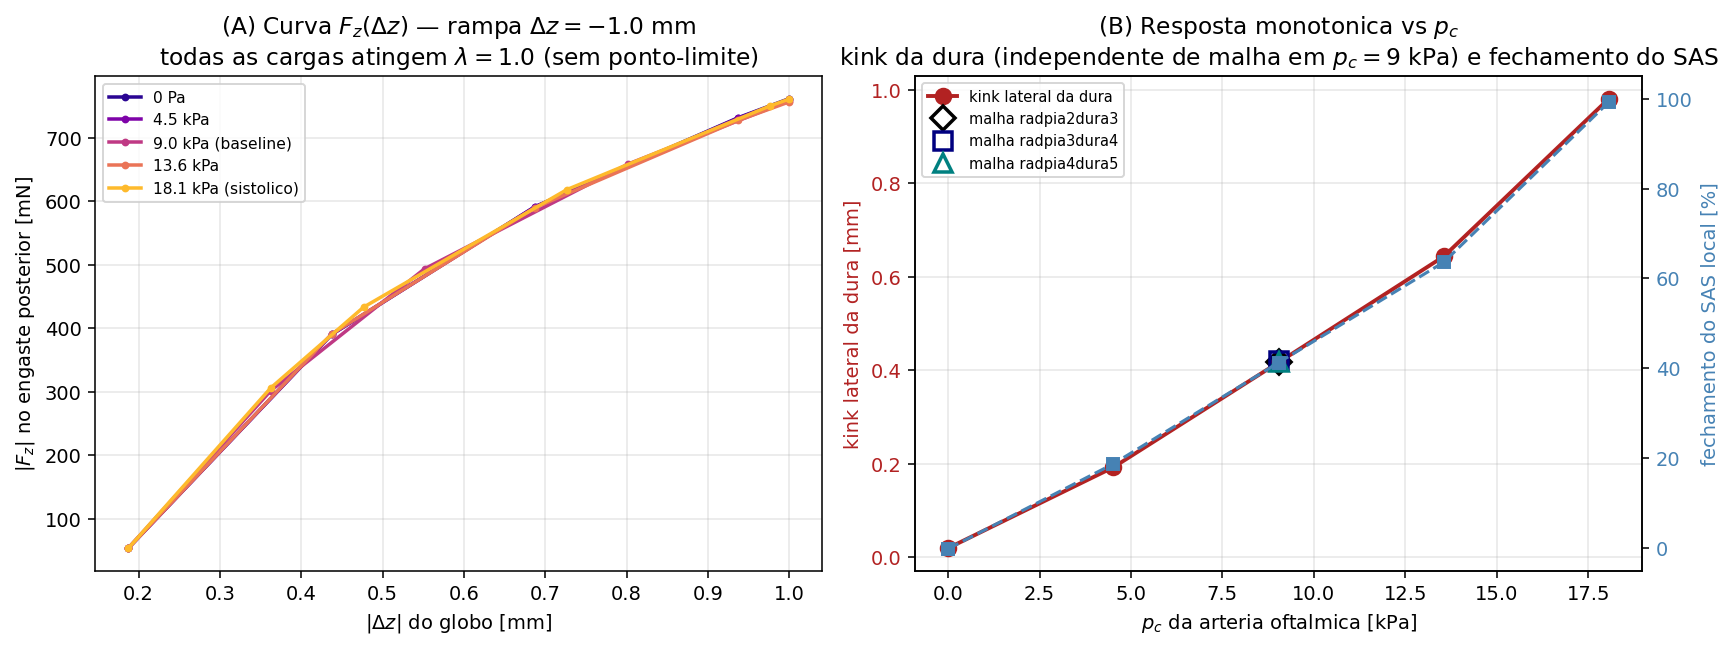
\includegraphics[width=0.95\linewidth]{on-caso-3f-dz1.png}
\caption{Caso 3F, rampa $\Delta z = -\SI{1.0}{\milli\meter}$. (A) Curvas $F_z(\Delta z)$ sobrepostas para os cinco valores de $p_c$: todas atingem $\lambda = 1{,}0$ de forma monotônica, sem ponto-limite. (B) Resposta monotônica em $p_c$: o $\mathrm{kink}$ lateral da dura (eixo esquerdo) e o fechamento do SAS local (eixo direito) crescem com a carga arterial; os três marcadores em $p_c = \SI{9}{\kilo\pascal}$ (malhas radiais) coincidem, atestando independência de malha.}
\label{fig:res-caso3f-dz1}
\end{figure}

\end{document}
